%%%%%%%%%%%%%%%%%%%%%%%%%%%%%%%%%%%%%%%%%
% Beamer Presentation
% LaTeX Template
% Version 1.0 (10/11/12)
%
% This template has been downloaded from:
% http://www.LaTeXTemplates.com
%
% License:
% CC BY-NC-SA 3.0 (http://creativecommons.org/licenses/by-nc-sa/3.0/)
%
%%%%%%%%%%%%%%%%%%%%%%%%%%%%%%%%%%%%%%%%%

%----------------------------------------------------------------------------------------
%	PACKAGES AND THEMES
%----------------------------------------------------------------------------------------

\documentclass{beamer}

\mode<presentation> {

% The Beamer class comes with a number of default slide themes
% which change the colors and layouts of slides. Below this is a list
% of all the themes, uncomment each in turn to see what they look like.

%\usetheme{default}
%\usetheme{AnnArbor}
%\usetheme{Antibes}
%\usetheme{Bergen}
%\usetheme{Berkeley}
%\usetheme{Berlin}
%\usetheme{Boadilla}
%\usetheme{CambridgeUS}
%\usetheme{Copenhagen}
%\usetheme{Darmstadt}
%\usetheme{Dresden}
%\usetheme{Frankfurt}
%\usetheme{Goettingen}
%\usetheme{Hannover}
%\usetheme{Ilmenau}
%\usetheme{JuanLesPins}
%\usetheme{Luebeck}
\usetheme{Madrid}
%\usetheme{Malmoe}
%\usetheme{Marburg}
%\usetheme{Montpellier}
%\usetheme{PaloAlto}
%\usetheme{Pittsburgh}
%\usetheme{Rochester}
%\usetheme{Singapore}
%\usetheme{Szeged}
%\usetheme{Warsaw}

% As well as themes, the Beamer class has a number of color themes
% for any slide theme. Uncomment each of these in turn to see how it
% changes the colors of your current slide theme.

%\usecolortheme{albatross}
%\usecolortheme{beaver}
%\usecolortheme{beetle}
%\usecolortheme{crane}
%\usecolortheme{dolphin}
%\usecolortheme{dove}
%\usecolortheme{fly}
%\usecolortheme{lily}
%\usecolortheme{orchid}
%\usecolortheme{rose}
%\usecolortheme{seagull}
%\usecolortheme{seahorse}
%\usecolortheme{whale}
%\usecolortheme{wolverine}

%\setbeamertemplate{footline} % To remove the footer line in all slides uncomment this line
%\setbeamertemplate{footline}[page number] % To replace the footer line in all slides with a simple slide count uncomment this line

\setbeamertemplate{navigation symbols}{} % To remove the navigation symbols from the bottom of all slides uncomment this line
}

\usepackage{graphicx} % Allows including images
\usepackage{booktabs} % Allows the use of \toprule, \midrule and \bottomrule in tables
\usepackage{subcaption}

\usepackage[backend=biber, style=reading]{biblatex}
\addbibresource{optimization.bib}

\usepackage{amsmath}
\usepackage{amssymb}
\usepackage{bbold}
\usepackage{mathrsfs}
\usepackage{bm}

\usepackage{algorithm}
\usepackage[noend]{algorithmic} 

\DeclareMathOperator{\Tr}{Tr}
\DeclareMathOperator{\cst}{cst}
\DeclareMathOperator{\Gram}{Gram}
\DeclareMathOperator{\R}{\mathbb{R}}
\DeclareMathOperator{\1}{\mathbb{1}}
\DeclareMathOperator{\E}{\mathbf{E}}
\DeclareMathOperator{\Y}{\mathcal{Y}}
\DeclareMathOperator*{\argmax}{arg\,max}
\DeclareMathOperator*{\argmin}{arg\,min}
\DeclareMathOperator{\dom}{Dom}

%----------------------------------------------------------------------------------------
%	TITLE PAGE
%----------------------------------------------------------------------------------------

\title[SDCA for CRF]{Stochastic Dual Coordinate Ascent for training Conditional Random Fields} % The short title appears at the bottom of every slide, the full title is only on the title page

\author{R\'emi Le Priol} % Your name
\institute[MILA] % Your institution as it will appear on the bottom of every slide, may be shorthand to save space
{
Montreal Institute of Learning Algorithms \\ % Your institution for the title page
\medskip
\textit{remi.lp.17@gmail.com} % Your email address
}
\date{\today} % Date, can be changed to a custom date

\begin{document}

\begin{frame}
\titlepage % Print the title page as the first slide
\end{frame}

\begin{frame}
\frametitle{Overview} % Table of contents slide, comment this block out to remove it
\tableofcontents % Throughout your presentation, if you choose to use \section{} and \subsection{} commands, these will automatically be printed on this slide as an overview of your presentation
\end{frame}

%----------------------------------------------------------------------------------------
%	PRESENTATION SLIDES
%----------------------------------------------------------------------------------------

%----------------------------------------------------------------------------------------
\section{Conditional Random Fields}
%----------------------------------------------------------------------------------------
\begin{frame}
	\frametitle{Overview}
	\tableofcontents[currentsection] 
\end{frame}
%----------------------------------------------------------------------------------------
\begin{frame}
\frametitle{Structured Prediction}

\begin{center}
	\begin{align*}
		\textrm{ data point } x \in \mathcal X & \mapsto \textrm{ structured label } y \in \Y \\
		\textrm{letter drawings} & \mapsto \textrm{word}  \\
		\textrm{sentence in English} & \mapsto \textrm{sentence in French}  \\
		\textrm{sentence} & \mapsto \textrm{parsing tree}  \\
		\textrm{natural image} & \mapsto \textrm{semantic segmentation}  \\
	\end{align*}

\visible<2->{
\begin{block}{Hypothesis}
	The conditional distribution $p(y | x)$ is Markov with respect to an undirected graphical model $G=(V,E)$.
\end{block}
}

\end{center}
\end{frame}
%----------------------------------------------------------------------------------------
\begin{frame}
\frametitle{Features}

Feature extractor:
\begin{equation*}
	F:\mathcal X \times \mathcal Y \rightarrow \R^d
\end{equation*}

\begin{block}{Hypothesis}
	\begin{equation*}
		F(x, y) =  \sum_{c\in \mathcal{C}} F_c(x, y_c)
	\end{equation*}
	where $\mathcal C$ is the set of maximal cliques of G.
\end{block}

\end{frame}
%----------------------------------------------------------------------------------------
\begin{frame}
\frametitle{The Model}

Conditional probability of y given x:
\begin{equation*}
	\label{primal probability}
	p(y | x ; w) := \frac{\exp(w^TF(x, y))}{\sum_{y' \in \mathcal{Y}} \exp(w^TF(x, y'))}
\end{equation*}

Standard approach to train CRF: Maximum Likelihood
\begin{equation*}
	\min_w \mathscr P(w)  = \frac{\lambda}{2}\|w\|^2 - \frac{1}{n}   \sum_{i=1}^{n} \log(p(y_i|x_i; w))
\end{equation*}

\end{frame}
%----------------------------------------------------------------------------------------
\begin{frame}
\frametitle{Reformulation}

New notations:
\begin{align*}
	&\textrm{Corrected features:} & \psi_i(y) := F(x_i, y_i) - F(x_i, y) \in \R^d \\
	&\textrm{Corrected feature matrix:} & A_i := ( \psi_i(1),\psi_i(2),...,\psi_i(|\Y_i|) ) \in \R^{d\times |\Y_i|} \\
	&\textrm{Log-sum-exp function:} & \phi_i(z) = \log \big(\sum_{y\in \Y_i} \exp(z_y)\big)
\end{align*}

\visible<2->{
The log-likelihood becomes :
\begin{align*}
	- \log(p(y_i|x_i; w)) 
	& = \log \big (\sum_y e^{w^TF(x_i, y)} \big ) - w^TF(x_i, y_i) \\
	& = \log \big (\sum_y e^{- w^T\psi_i(y)} \big ) \\
	& = \phi_i(-A_i^Tw)
\end{align*}
}
\end{frame}
%----------------------------------------------------------------------------------------
\begin{frame}
\frametitle{Primal Objective}

\begin{equation}
	\min_{w\in\R^d}  \mathscr P(w) = \frac{\lambda}{2}\|w\|^2 + \frac{1}{n}   \sum_{i=1}^{n} \phi_i(-A_i^Tw)
\end{equation}

\begin{center}
	\visible<2->{HARD ! $A_i$ is huge.} 
\end{center}


\end{frame}
%----------------------------------------------------------------------------------------
\begin{frame}[fragile]
	\frametitle{Anterior Work}
	\begin{itemize}
		\item Exponentiated Gradient by Collins in 2008 \footcite{collins_exponentiated_2008}
		\item Non-Uniform Sampling -- Stochastic Average Gradient (NUS-SAG) by Schmidt in 2014 \footcite{schmidt_non-uniform_2015}
		\item<2-> SDCA \footcite{shalev-shwartz_accelerated_2013-1}
	\end{itemize}


\begin{center}
	\visible<3->{Variance reduced methods.\\}
	\bigskip
	\visible<4->{Why SDCA?\\}
	\bigskip
	\visible<5->{\textbf{Exact line search for cheap!}}
\end{center}




\end{frame}
%----------------------------------------------------------------------------------------
%\begin{frame}
%\frametitle{Why SDCA?}
%\begin{center}
%$L =$ smoothness of $\mathcal P$, 
%$m =$ strong convexity of $\mathcal P$, 
%$\lambda \leq m \leq L$\\
%\bigskip
%\begin{tabular}{clclc}
%Algorithm & Convergence rate & Guarantee \\
%\hline
%Online EG & $O((n + \frac{L}{\lambda})\log(1/\epsilon))$ & (dual)\\
%SAG & $O((n + \frac{L}{m})\log(1/\epsilon))$ & (primal) \\
%SDCA & $O( (n + \min( \frac{L}{\lambda}, \sqrt{\frac{n L}{\lambda}}) ) \log(1/\epsilon) )$ & (duality gap)
%\end{tabular}
%
%\bigskip
%
%\visible<2->{Not a better rate, but...}
%
%\bigskip
%
%\visible<3->{\textbf{Exact line search for cheap!}}
%
%\end{center}
%
%
%\end{frame}
%----------------------------------------------------------------------------------------
\section{SDCA for Max-likelihood}
%----------------------------------------------------------------------------------------
\begin{frame}
	\frametitle{Overview}
	\tableofcontents[currentsection] 
\end{frame}
%----------------------------------------------------------------------------------------
%\begin{frame}
%\frametitle{Empirical Risk Minimization and its Dual}
%General setting of SDCA: \\
%Regularizer $R$, loss functions $\phi_i$, feature matrices $A_i$.
%
%Primal 
%\begin{equation}
%	\min_{w\in\R^d}  R(w) + \frac{1}{n}   \sum_{i=1}^{n} \phi_i(-A_i^Tw)
%\end{equation}
%
%Dual
%\begin{equation*}
%	\max_{\alpha | \forall i, \alpha_i \in \dom \phi_i^*} \   -  \frac{1}{n} \sum_i A_i \alpha_i \|^2 + \frac{1}{n} \sum_i -\phi_i^*(\alpha_i) 
%\end{equation*}
%
%SDCA update:
%\begin{equation}
%	\alpha_i^+ \leftarrow (1-\gamma) \alpha_i + \gamma \nabla \phi_i(-\frac{1}{\lambda n} A_i^TA\alpha) \quad \textrm{with} \quad \gamma \in [0, 1]
%\end{equation}
%
%\end{frame}
%----------------------------------------------------------------------------------------
\begin{frame}
\frametitle{Dual Formulation}

Primal:
\begin{equation*}
	\min_{w\in\R^d}  \frac{\lambda}{2}\|w\|^2 + \frac{1}{n}   \sum_{i=1}^{n} \phi_i(-A_i^Tw)
\end{equation*}

Dual:
\begin{equation*}
	\max_{\alpha | \forall i, \alpha_i \in \Delta_i} \mathscr{D}(\alpha) = -\frac{1}{2\lambda} \| \frac{1}{n} \sum_i A_i \alpha_i \|^2 + \frac{1}{n} \sum_{i=1}^n H_i(\alpha_i)
\end{equation*}
$\Delta_i$ is the simplex of dimension $|\Y_i|$.
$H_i$ is the entropy over $\Delta_i$.

\end{frame}
%----------------------------------------------------------------------------------------
\begin{frame}
\frametitle{Conjugate variables}

Primal probabilities
\begin{equation*}
	\label{primal to dual}
	\forall i, \bm \alpha_i(w) := \nabla\phi_i(-A_i^Tw) = p(.|x_i; w) \propto \exp(-w^T \psi_i(.))
\end{equation*}

Dual weights
\begin{align*}
	\label{dual to primal}
	\bm w(\alpha) 
	& =   \frac{1}{\lambda n} \sum_i A_i \alpha_i = \frac{1}{\lambda n} \sum_i \E_{\alpha_i} [\psi_i] \\
	& =\frac{1}{\lambda n} \sum_i F(x_i, y_i) - \frac{1}{\lambda n} \sum_i \E_{y \sim \alpha_i} [F(x_i, y)]
\end{align*}

\visible<2->{
\begin{block}{Optimality condition}
	\begin{equation*}
		\alpha^* = \bm \alpha(w^*) \quad \textrm{and} \quad w^* = \bm w(\alpha^*)
	\end{equation*}
\end{block}
}

\end{frame}
%----------------------------------------------------------------------------------------
\begin{frame}
	\frametitle{Max-entropy}
	
\begin{equation*}
	\max_{\alpha | \forall i, \alpha_i \in \Delta_i} \mathscr{D}(\alpha) = \underbrace{-\frac{\lambda}{2} \| \bm w(\alpha) \|^2}_\text{data fitting} + \underbrace{ \frac{1}{n} \sum_{i=1}^n H_i(\alpha_i)}_\text{regularization}
\end{equation*}

\begin{center}
	\visible<2->{HARD ! $\alpha$ is huge.} 
\end{center}
	
\end{frame}
%----------------------------------------------------------------------------------------
\begin{frame}
\frametitle{Principle of SDCA\footcite{shalev-shwartz_accelerated_2013-1}}
\begin{itemize}
	\item Store dual probabilities $\alpha$ and $\bm w(\alpha)$.
	\item Sample $i \in \{1,\dots ,n\}$
	\item Update $\alpha_i^+ \leftarrow (1-\gamma) \alpha_i + \gamma \bm \alpha_i(\bm w(\alpha))$ with $\gamma \in [0, 1]$
\end{itemize}

\end{frame}
%----------------------------------------------------------------------------------------
\begin{frame}[fragile]
\frametitle{Pseudo code}

\begin{algorithm}[H]
    \caption{SDCA for Logistic Regression}
    \label{sdca for logreg}
\begin{algorithmic}
        %
        \STATE $\forall i,$ initialize $\alpha_i^{(0)}$ at random in $\Delta_K$
        \STATE Let $w^{(0)} = \frac{1}{\lambda n} A \alpha$  
        \STATE Let $\forall i,\  g_i = 1$ (optional)
        %
       \FOR{$k=0\dots K$}
                \STATE Pick $i$ at random in $\{1,\ldots,n\}$ (optionally, proportional to $g_i$)
                \STATE Let $ \beta_i := p( . |x ; w^{(k)}) = \bm \alpha_i(\bm w(\alpha_i^{(k)}))$ 
                %
                \STATE Let $g_i = D_{KL}(\alpha_i || \beta_i)$ (optional)
                %
                \STATE Let $d_i = \beta_i - \alpha_i^{(k)}$ (dual ascent direction)
                \STATE Let $v_i = \frac{1}{\lambda n} A_i d_i $ (primal descent direction)
                \STATE Solve $\gamma^* = \argmax_{\gamma \in [0,1]} H_i(\alpha_i^{(k)} + \gamma d_i) - \frac{\lambda n}{2} \| w^{(k)} + \gamma v_i \|^2$ (Line Search)
                %
               \STATE Update $\alpha_i^{(k+1)} := \alpha_i^{(k)} + \gamma^* d_i$
               \STATE Update $w^{(k+1)} := w^{(k)} + \gamma^* v_i $
        \ENDFOR
\end{algorithmic}
\end{algorithm}
% Insist on the fact that we need to evaluate the conjugate variable only one. 
% Going from one to the other is the bottleneck step.
\end{frame}
%----------------------------------------------------------------------------------------
%----------------------------------------------------------------------------------------
\section{Non-Uniform Sampling}
%----------------------------------------------------------------------------------------
\begin{frame}
	\frametitle{Overview}
	\tableofcontents[currentsection] 
\end{frame}
%----------------------------------------------------------------------------------------
\begin{frame}
	\frametitle{On duality gaps}
	Duality gap:
	\begin{equation*}
		g(w,\alpha) = \mathscr P(w) - \mathscr D(\alpha)
	\end{equation*}
	
	Primal model gap:
	\begin{equation*}
		\label{primal duality gap}
		g(w,\bm \alpha(w)) = \frac{\lambda}{2} \|w- \bm w(\bm \alpha(w))\|^2 = \frac{1}{2 \lambda} \|\nabla \mathscr P(w)\|^2
	\end{equation*}
	
	Dual model gap:
	\begin{equation*}
		g(\bm w(\alpha),\alpha) = \frac{1}{n} \sum_i D_{KL} (\alpha_i || \bm \alpha_i(\bm w(\alpha))
	\end{equation*}
	
\end{frame}
%----------------------------------------------------------------------------------------
\begin{frame}
	\frametitle{Idea}
	
	\begin{block}{Our Scheme}
	\begin{itemize}
		\item At each step, update individual duality gap $ g_i = D_{KL} (\alpha_i || \bm \alpha_i(\bm w(\alpha))$
		\item Sample $i$ proportionally to $g_i$.
	\end{itemize}
	\visible<2->{
	Scheme adapted from Block-Coordinate Franck-Wolfe\footcite{osokin_minding_2016}.\\
	Transposable to the exponentiated gradient.
	}
	\end{block}
	
	\visible<3->{
	\begin{block}{Competing scheme}
	\begin{equation*}
		g_i =  \| \bm \alpha_i(\bm w(\alpha)) - \alpha_i \|  \sqrt{R_i^2 + 2 \lambda n} 
	\end{equation*}
	where $R_i$ is the operator norm of $A_i$.\footcite{csiba_stochastic_2015}
	\end{block}
	}
	
\end{frame}

%----------------------------------------------------------------------------------------
\begin{frame}
	\frametitle{Results 1}
	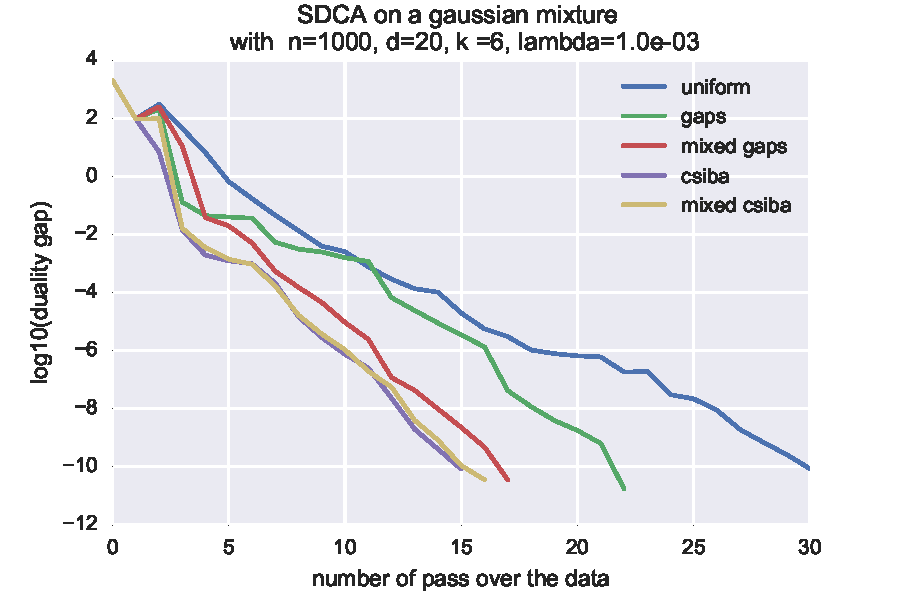
\includegraphics[width=\textwidth]{images/20170914_061831_gaussians_perf}
\end{frame}
%----------------------------------------------------------------------------------------
\begin{frame}
	\frametitle{Results 2}
	% Covertype dataset. 7 classes in dimension 55. 
	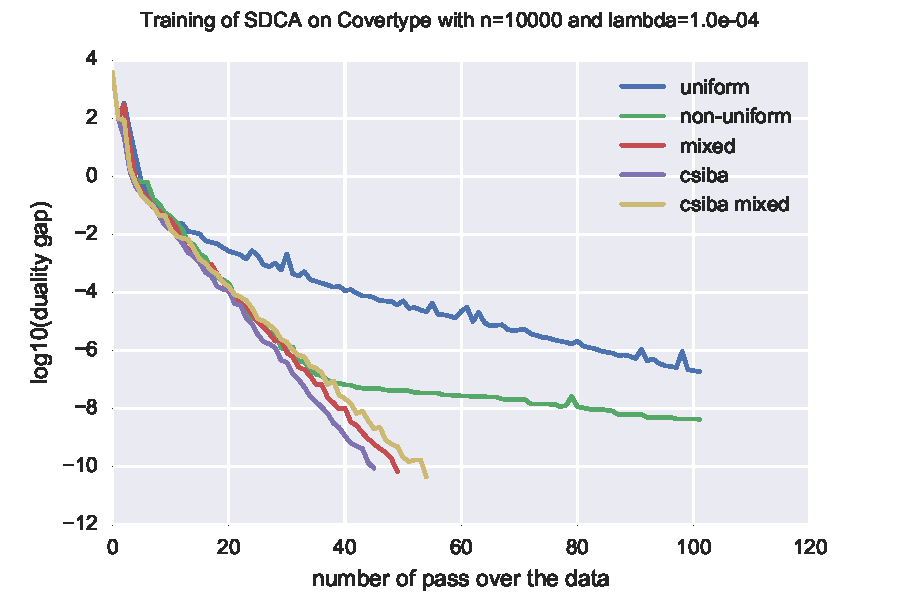
\includegraphics[width=\textwidth]{images/20170914_065817_covertype_perf}
	% Show a plot where the uniform scheme actually has access to as much data as the non-uniform ones.
	% Csiba's scheme is marginally better, but it does not scale to structured CRF
\end{frame}
%----------------------------------------------------------------------------------------
%----------------------------------------------------------------------------------------
\section{Leverage the Structure}
%----------------------------------------------------------------------------------------
\begin{frame}
	\frametitle{Overview}
	\tableofcontents[currentsection]  
\end{frame}
%----------------------------------------------------------------------------------------
\begin{frame}[fragile]
	\frametitle{Joints and Marginals \footcite{taskar_max-margin_2004} }
	
	Marginal probability on the clique $c \in \mathcal C$.
	\begin{equation*}
	\label{marginals definition}
	\mu_{i, c}(y_c) := \sum_{y'\in \Y_i | y_c' = y_{i, c}} \alpha_i(y')
	\end{equation*}
	The marginals of the sample i live in the local consistency polytope $L_i$.
	
	If $\mathcal T = (\mathcal C, \mathcal S)$ is a junction tree of $G$:
	\begin{equation}
		\label{joint from marginals}
		\alpha(y) = \frac{\prod_{c\in\mathcal{C}_{max}} \mu_c(y_c)}{\prod_{s\in\mathcal{S}} \mu_s(y_s)}
	\end{equation}
	Junction Tree algorithm = marginalization oracle.
	\begin{center}
		We can compute $p_c(y_c | x_i ; w) = \mu_{i,c}'(y_c)$.
	\end{center}

\end{frame}
%----------------------------------------------------------------------------------------
\begin{frame}
	\frametitle{Marginals to the Weights}	
	
	\begin{align*}
	\bm w(\alpha)
	& = \frac{1}{\lambda n} \sum_i \E_{y \sim \alpha_i}[\psi_i(y)] \\
   	&  = \frac{1}{\lambda n} \sum_i \sum_{c \in \mathcal C_i} \E_{y \sim \alpha_i}  [\psi_{i, c}(y_c)]  \\
   	&  = \frac{1}{\lambda n} \sum_i \sum_{c \in \mathcal C_i} \E_{y_c \sim \mu_{i, c}}  [\psi_{i, c}(y_c)] 
	\end{align*}

\begin{block}{Marginal weights}
	\begin{equation*}
		\mathcal W (\mu) := \frac{1}{\lambda n} \sum_i \sum_c B_{i, c} \mu_{i, c}
	\end{equation*}
	where $B_{i, c}$ has size $d\times |\Y_c|$, with $\psi_{i, c}(y_c)$ in the column $y_c$.
\end{block}
	
\end{frame}
%----------------------------------------------------------------------------------------
\begin{frame}
	\frametitle{Marginals to the Entropy}
	
	We express the entropy of the joint probability as a function of the marginals with equation \ref{joint from marginals}.
	\begin{align*}
	%\label{marginals entropy}
	\mathcal H (\mu) := H_{|\Y|} (\alpha) & = \sum_c H_{|c|}(\mu_c) - \sum_s H_{|s|}(\mu_s) \\
	%\label{marginals divergence}
	\mathcal D (\mu||\mu') := D_{KL}(\alpha||\alpha') & = \sum_c D(\mu_c||\mu_c') - \sum_s D(\mu_s||\mu_s')
	\end{align*}
	
	\textit{Remark:} We can directly transpose our non-uniform sampling scheme.
	This is not true for Cisba's scheme.

\end{frame}
%----------------------------------------------------------------------------------------
\begin{frame}
	\frametitle{A New Dual Objective}
	
	\begin{equation}
	\max_{\forall i, \mu_i \in \mathcal L_i} - \frac{\lambda}{2} \| \mathcal W(\mu)\|^2 + \frac{1}{n} \sum_i \mathcal H _ i(\mu_i)
	\end{equation}
	
	\begin{center}
		We apply the coordinate ascent directly on this objective
	\end{center}

\end{frame}
%----------------------------------------------------------------------------------------
\begin{frame}[fragile]
	\frametitle{Pseudo Code}
	
	\begin{algorithm}[H]
    	\caption{SDCA for CRF}
    	\label{sdca for crf}	
    \begin{algorithmic}
        \STATE Let $\forall i, c, \mu_{i, c}^{(0)} := \frac{1}{|c|}$ and $w^{(0)} := \frac{1}{\lambda n} B \mu^{(0)} $
        \STATE Let $\forall i g_i = 1$ (optional)
        %
       \FOR{$k=0\dots K$}
                \STATE Pick $i$ at random in $\{1,\ldots,n\}$ (optionally, proportional to $g_i$)
                \STATE Compute $\forall c, \mu_{i, c}' (y_c) := p(y_c|x; w^{(k)})$ (marginalization oracle)
                %
                \STATE Let $g_i = \mathcal D(\mu_i || \mu_i')$ (optional)
                %
                \STATE Let $d_i = \mu_i' - \mu_i^{(k)}$ (ascent direction)
                \STATE Let $v_i = \frac{1}{\lambda} B_i d_i $ (primal direction)
                \STATE Solve $\gamma^* = \argmax_{\gamma \in [0,1]} \mathcal H_i(\mu_i^{(k)} + \gamma d_i) - \frac{\lambda n}{2} \| w^{(k)} + \frac{\gamma}{n} v_i \|^2$ (Line Search)
                %
               \STATE Update $\mu_i^{(k+1)} := \mu_i^{(k)} + \gamma^* d_i$
               \STATE Update $w^{(k+1)} := w^{(k)} + \frac{\gamma^*}{n} v_i $
        \ENDFOR
	\end{algorithmic}
	\end{algorithm}

\end{frame}
%----------------------------------------------------------------------------------------
\begin{frame}
	\frametitle{Results 1}
	\begin{center}	
		No convergence yet.\\
		\bigskip
		\includegraphics<1>[width=\textwidth,height=0.8\textheight,keepaspectratio]{images/20170914_040237_ocr_perf.pdf}
        \includegraphics<2>[width=\textwidth,height=0.8\textheight,keepaspectratio]{images/20170914_041643_ocr_perf.pdf}
        \includegraphics<3>[width=\textwidth,height=0.8\textheight,keepaspectratio]{images/20170914_040715_ocr_perf.pdf}
	\end{center}
\end{frame}
%----------------------------------------------------------------------------------------
\begin{frame}
	\begin{figure}
    \centering
    \begin{subfigure}[t]{0.3\textwidth}
        \centering
        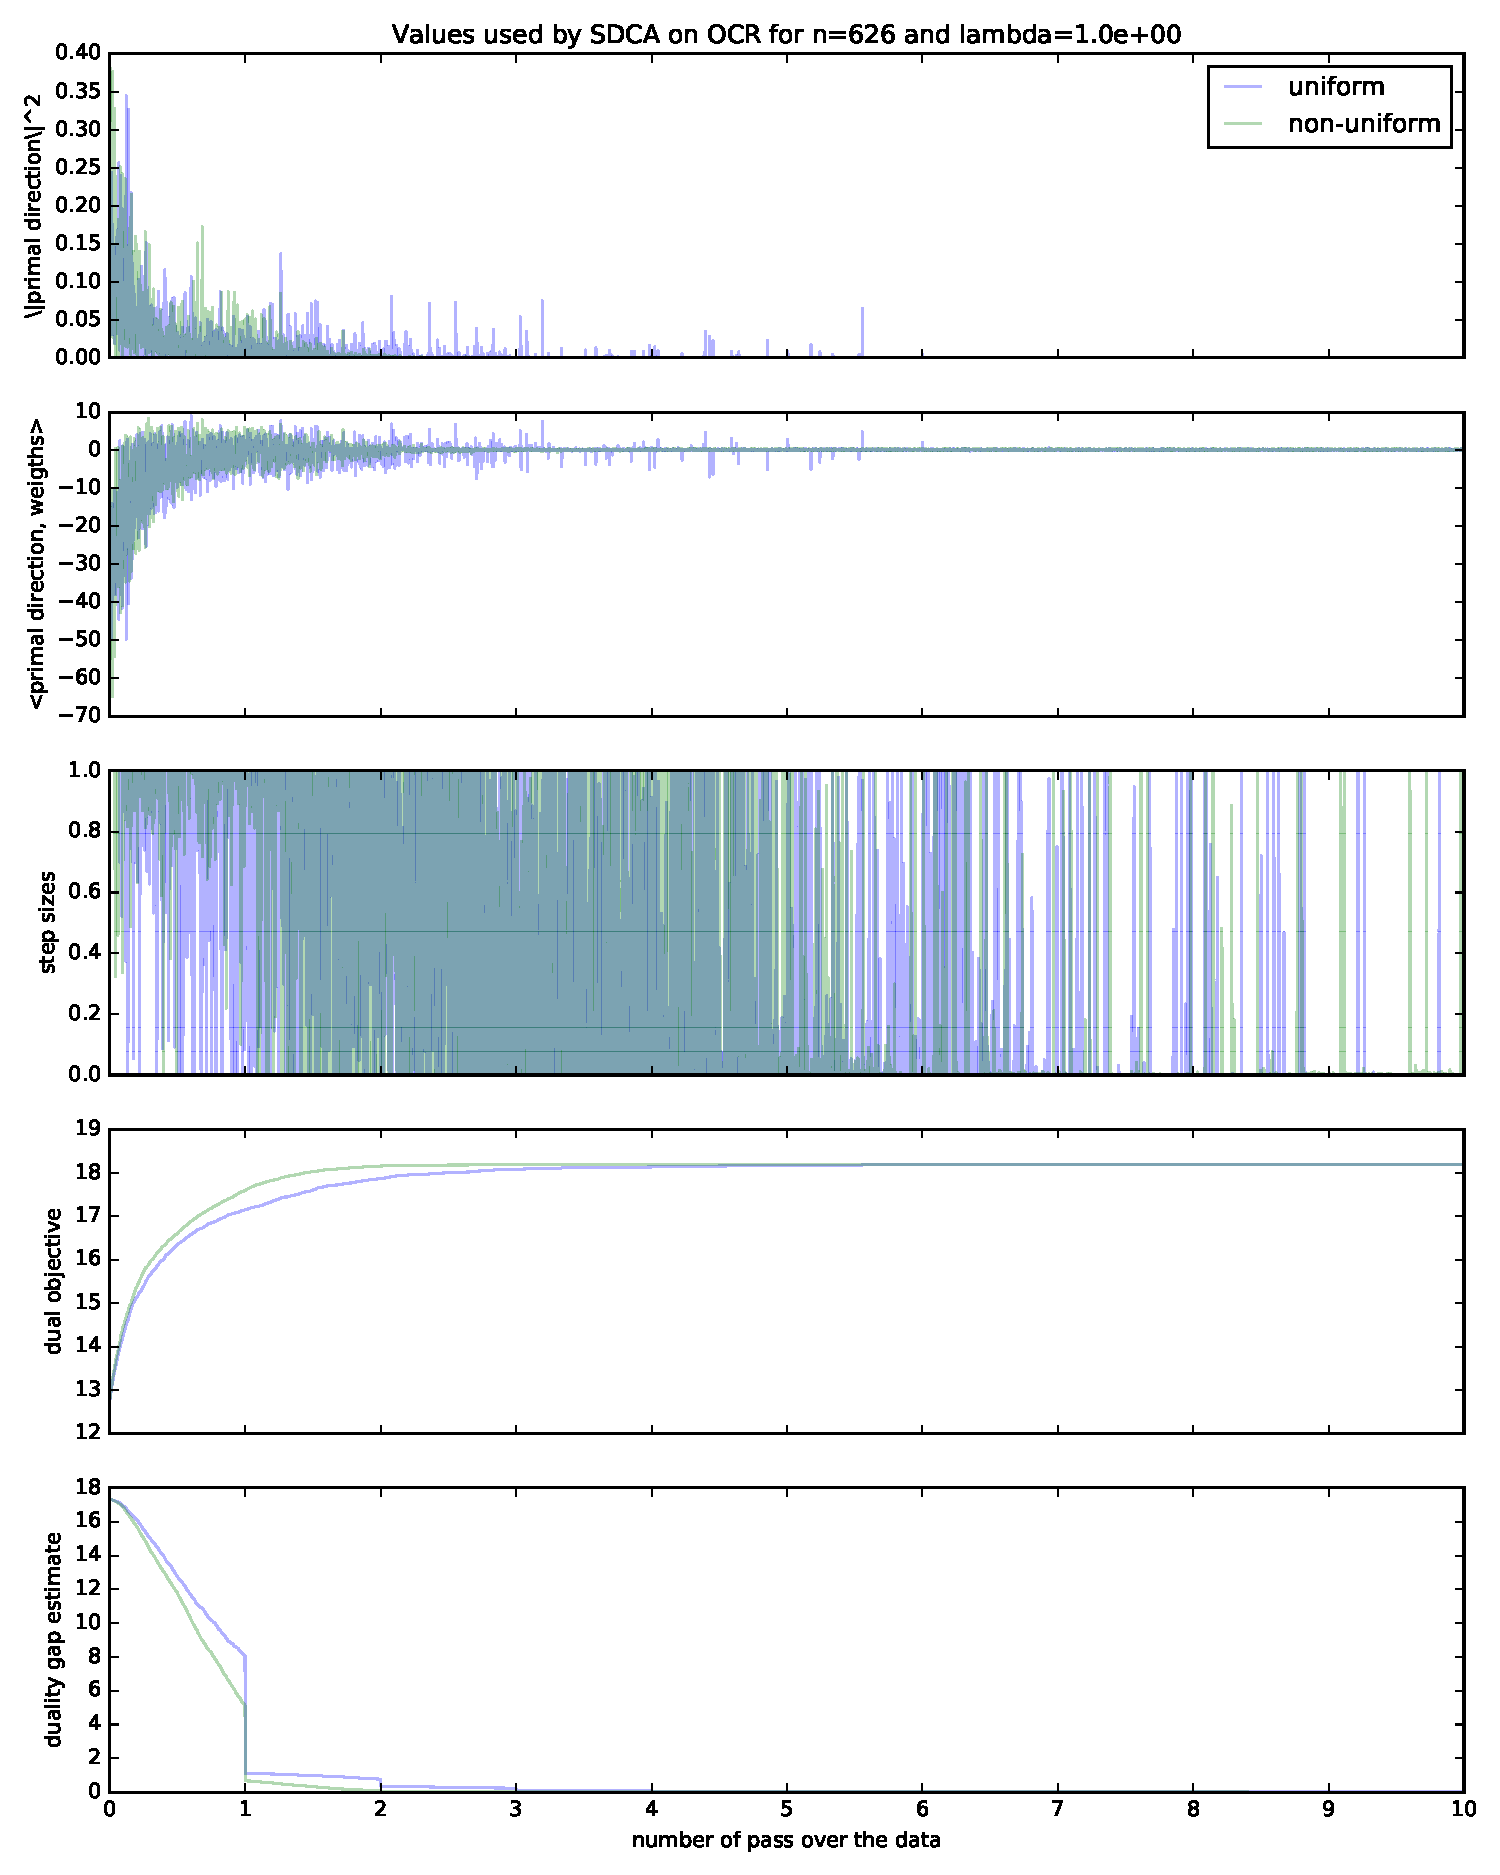
\includegraphics[width=\textwidth]{images/20170914_040249_ocr_annex.pdf}
    \end{subfigure}
    ~
    \begin{subfigure}[t]{0.3\textwidth}
        \centering
        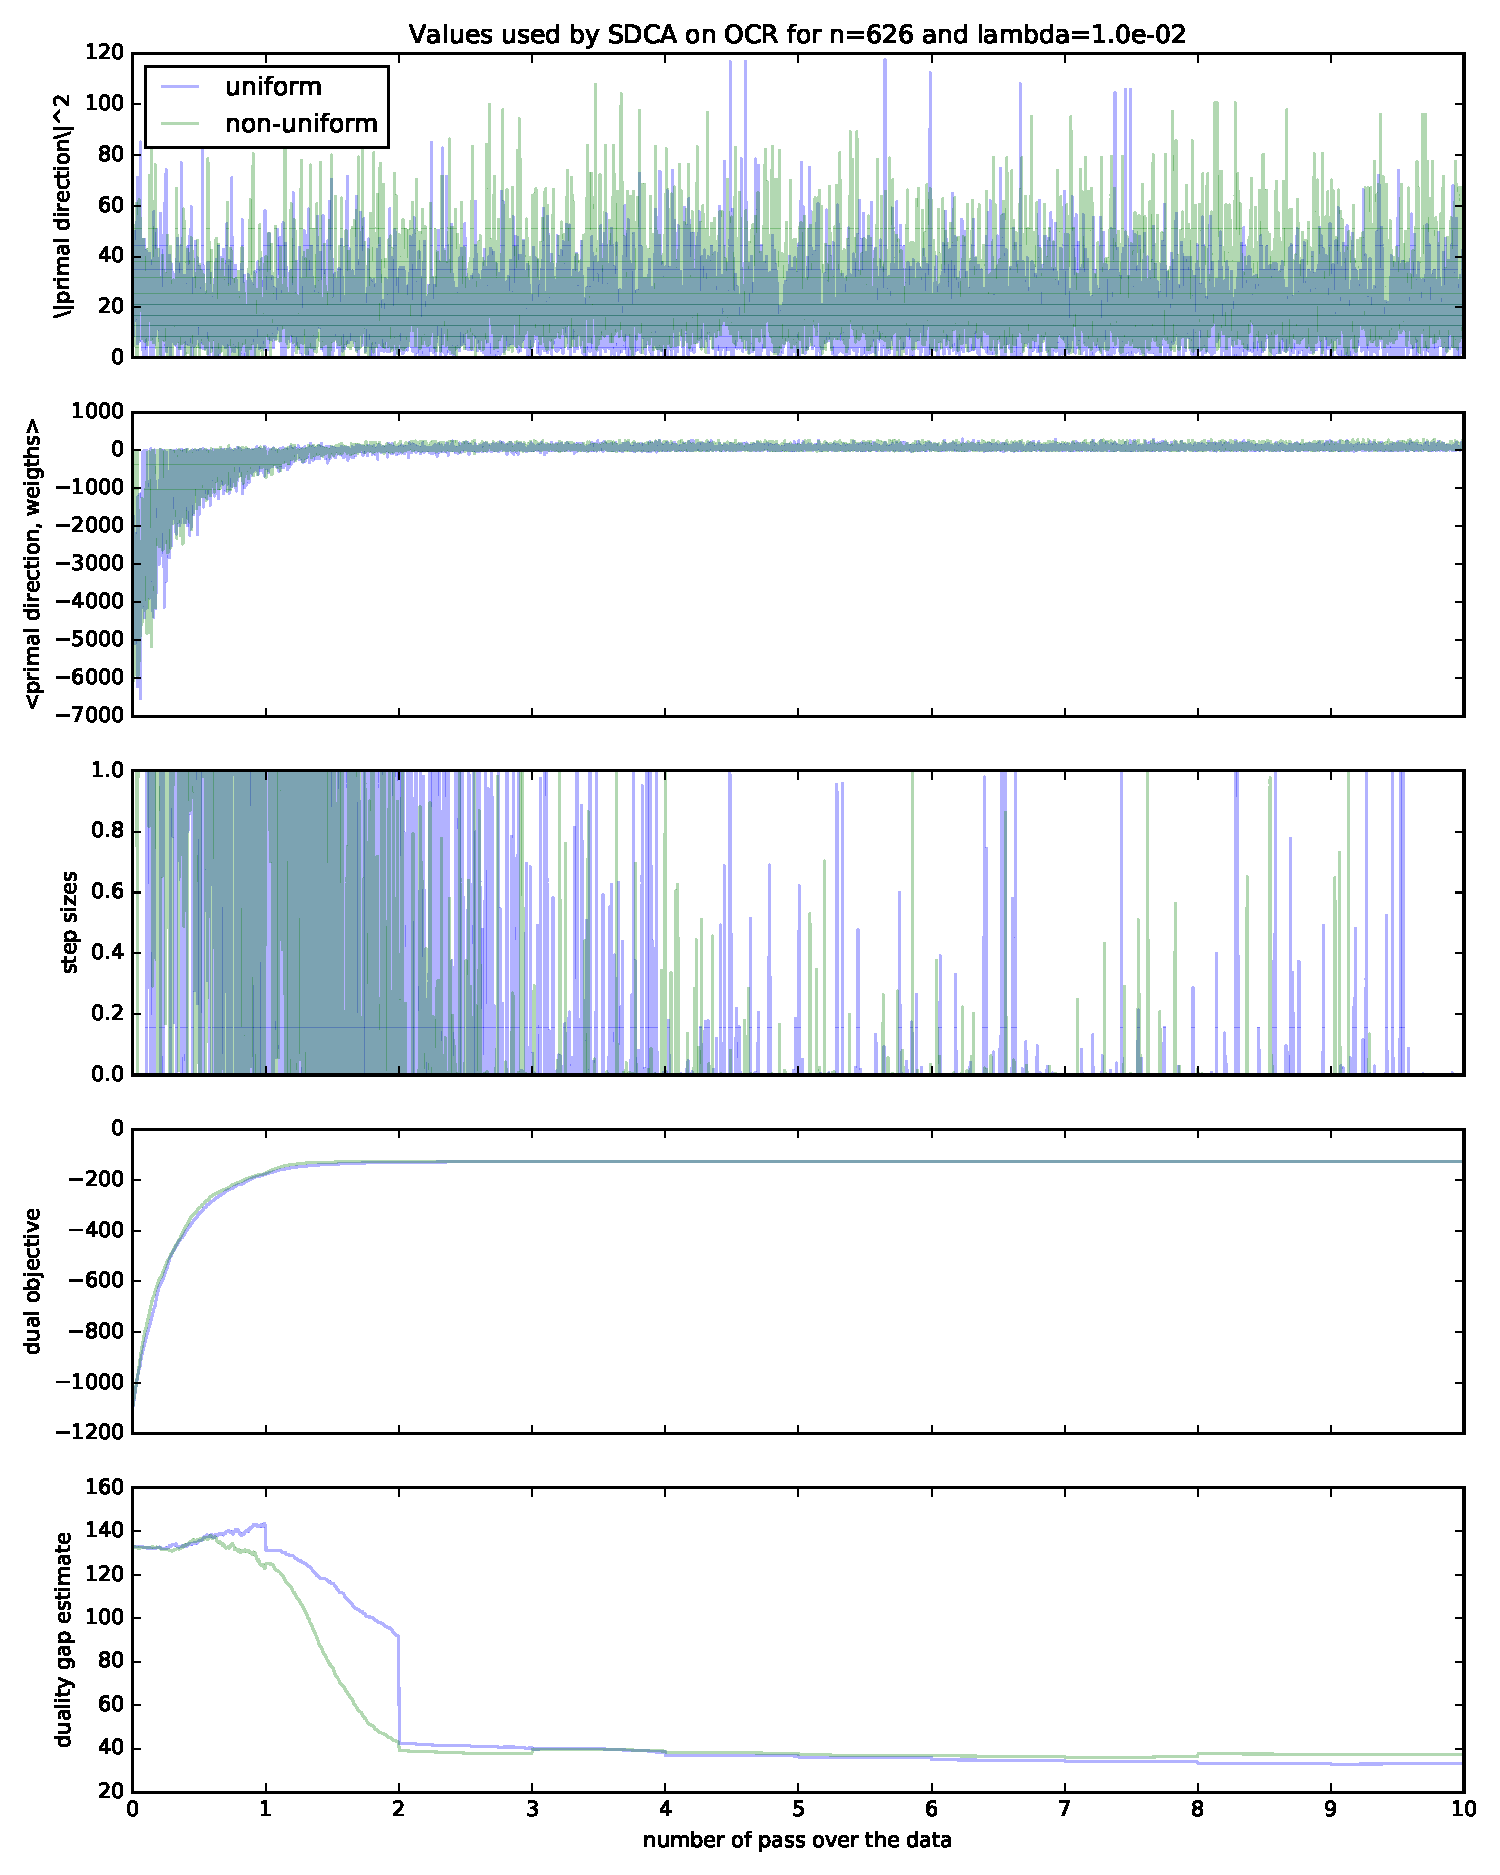
\includegraphics[width=\textwidth]{images/20170914_041645_ocr_annex.pdf}
    \end{subfigure}
    ~
    \begin{subfigure}[t]{0.3\textwidth}
        \centering
        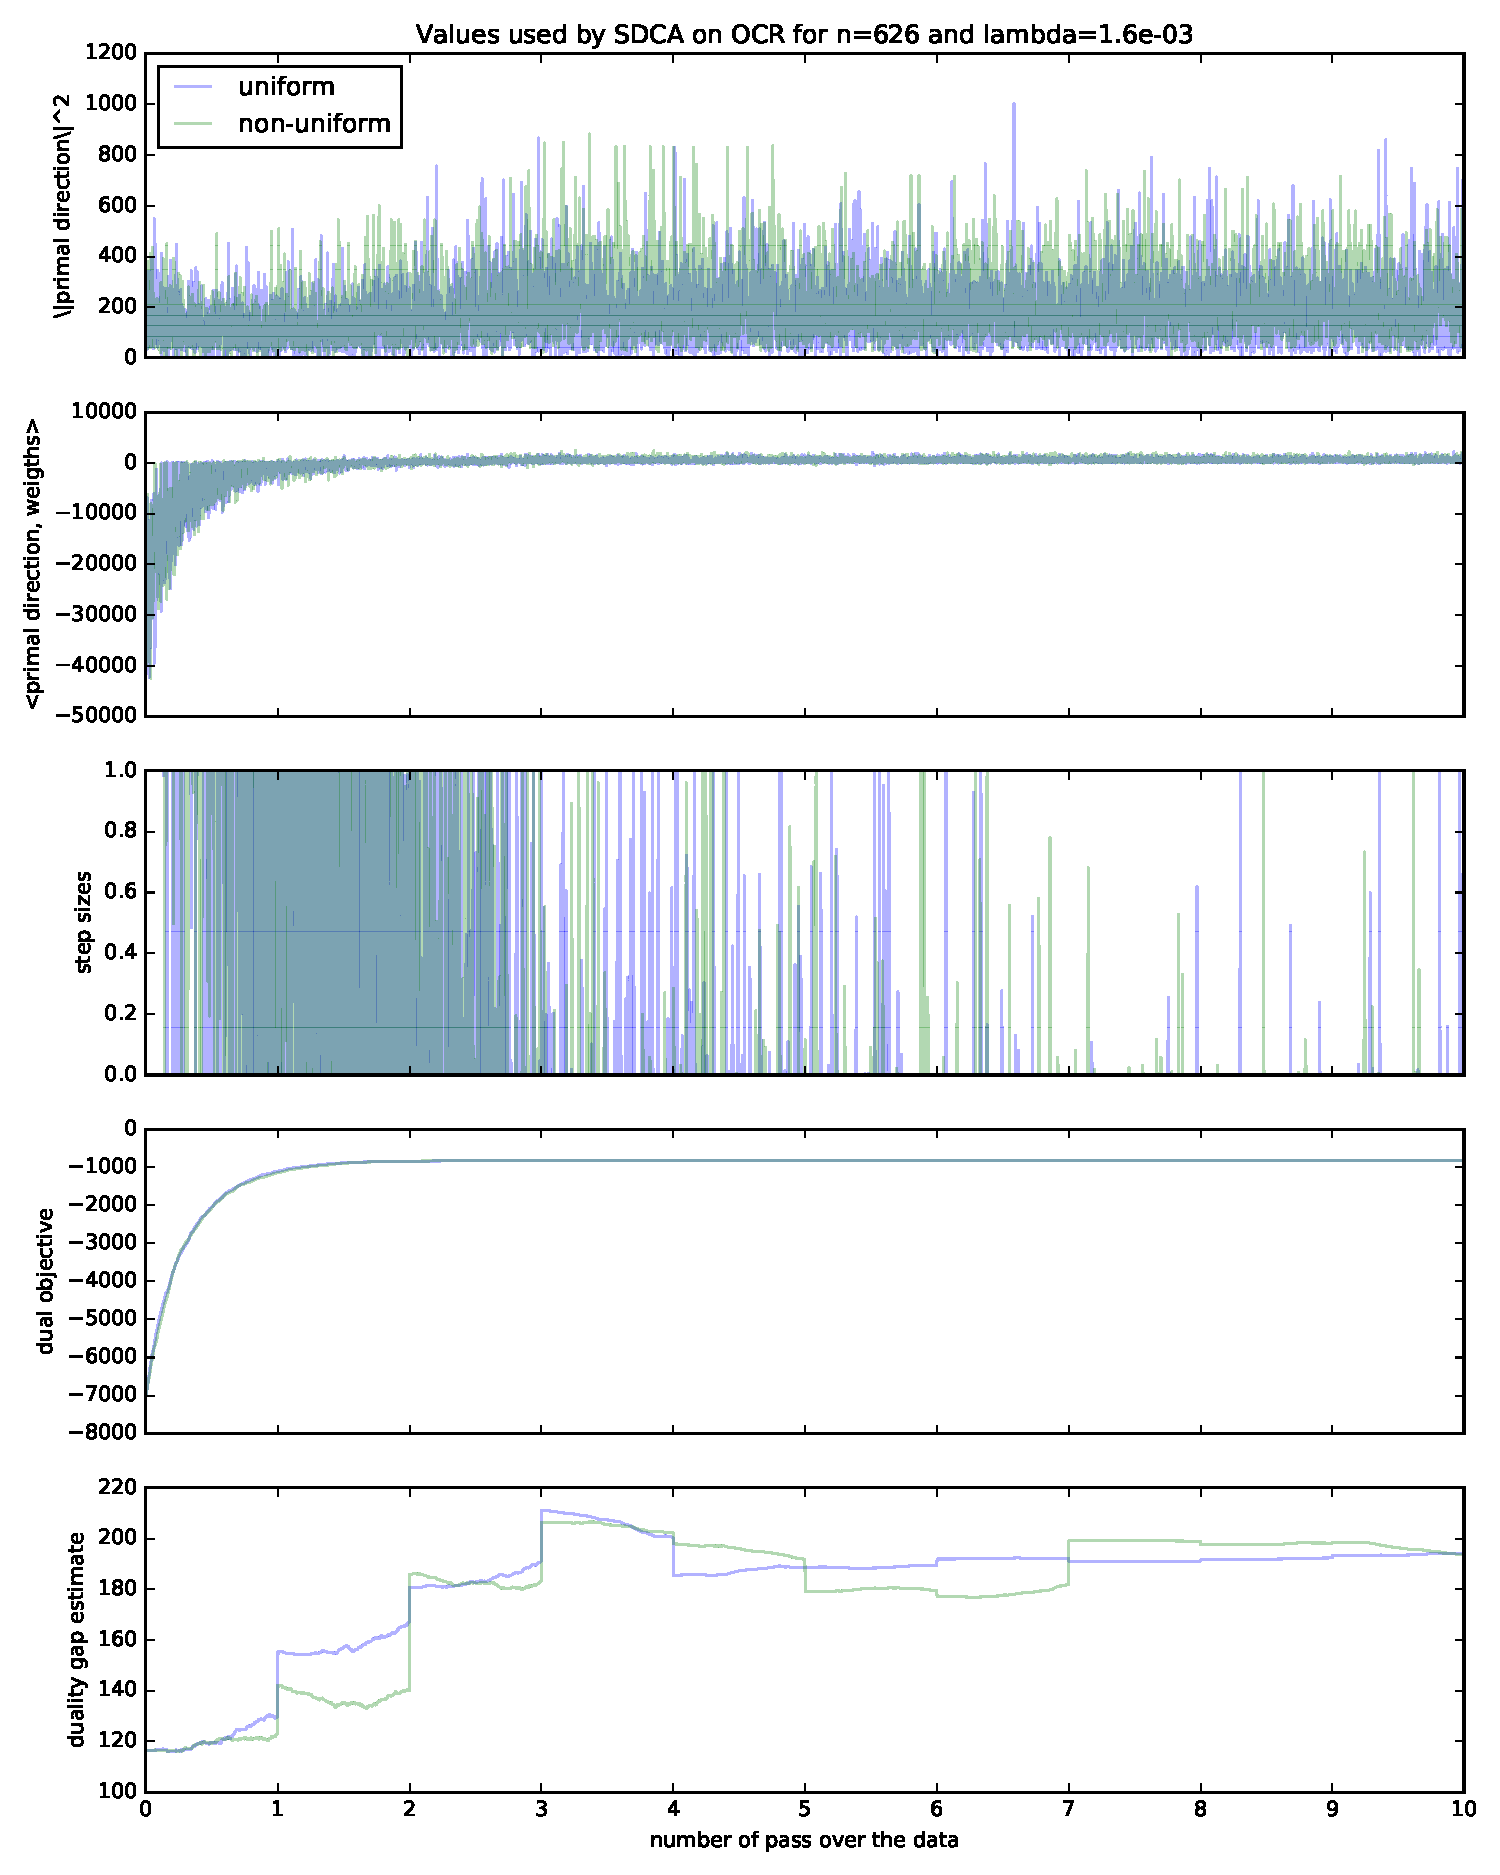
\includegraphics[width=\textwidth]{images/20170914_040717_ocr_annex}
    \end{subfigure}
    \caption{Some values of interest tracked along the run of SDCA.}
	\label{ocr annexes}
\end{figure}
\end{frame}
%----------------------------------------------------------------------------------------
\begin{frame}
\Huge{\centerline{Questions?}}
\end{frame}
%----------------------------------------------------------------------------------------
%----------------------------------------------------------------------------------------
%\begin{frame}
%	\printbibliography
%\end{frame}
%----------------------------------------------------------------------------------------
%----------------------------------------------------------------------------------------
\appendix
%----------------------------------------------------------------------------------------
\begin{frame}
	\frametitle{Appendix 1}
	\begin{figure}
	\center
	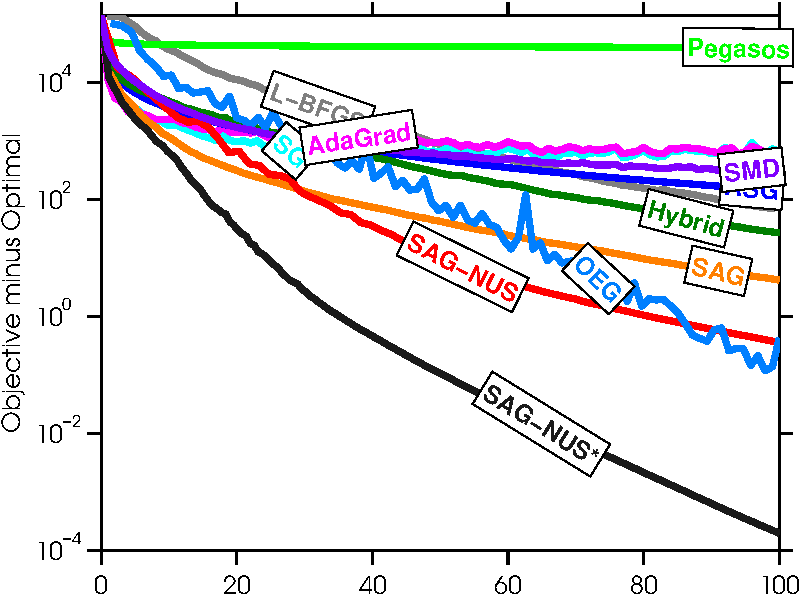
\includegraphics[width=.5\textwidth]{images/ocr2_train_passes.pdf}
	\caption{Training curves for various optimization algorithms on the OCR dataset. The x axis is the number of epochs, while the y axis is the primal suboptimality.}
	\label{schmidt's curves}
	\end{figure}
\end{frame}
%----------------------------------------------------------------------------------------
\begin{frame}
	\frametitle{Appendix 1}
	\begin{figure}
    \centering
    \begin{subfigure}[t]{0.3\textwidth}
        \centering
        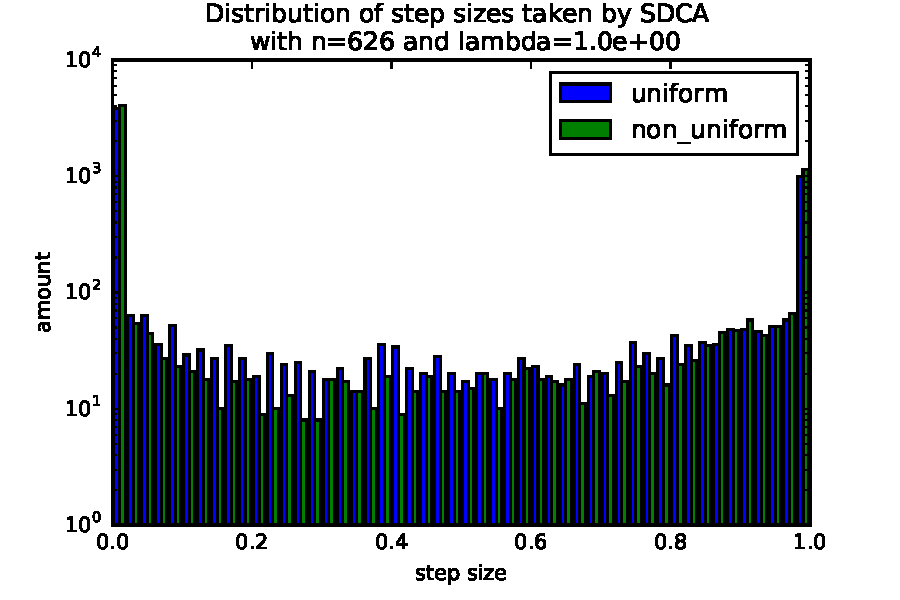
\includegraphics[width=\textwidth]{images/20170914_040255_ocr_stepdistrib.pdf}
    \end{subfigure}
    ~
    \begin{subfigure}[t]{0.3\textwidth}
        \centering
        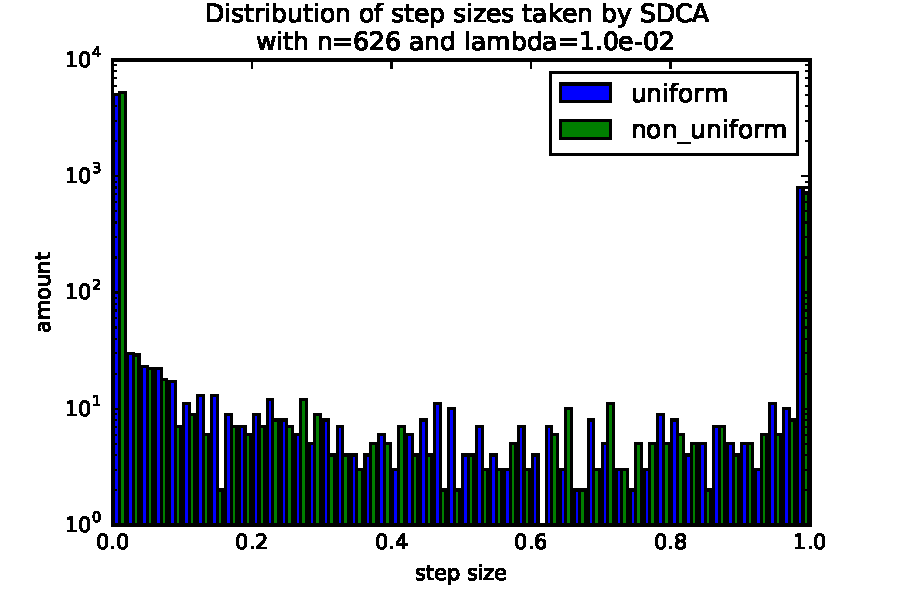
\includegraphics[width=\textwidth]{images/20170914_041649_ocr_stepdistrib.pdf}
    \end{subfigure}
    ~
    \begin{subfigure}[t]{0.3\textwidth}
        \centering
        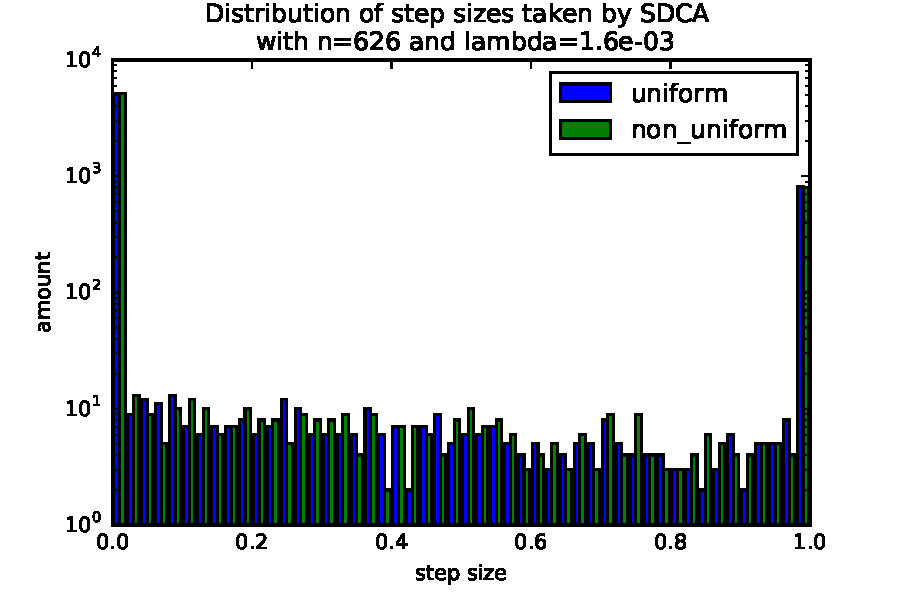
\includegraphics[width=\textwidth]{images/20170914_040720_ocr_stepdistrib.pdf}
    \end{subfigure}
    \caption{Distributions of step sizes taken by SDCA. The y axis is a log-scale. A large majority of steps are either taken with full size 1, either not taken at all. When the algorithm works better, with $\lambda$ large, there are more intermediate step sizes.}
	\label{ocr step sizes}
\end{figure}
\end{frame}
%----------------------------------------------------------------------------------------
\begin{frame}
	\frametitle{Appendix 1}
	\begin{figure}
    \centering
    \begin{subfigure}[t]{0.3\textwidth}
        \centering
        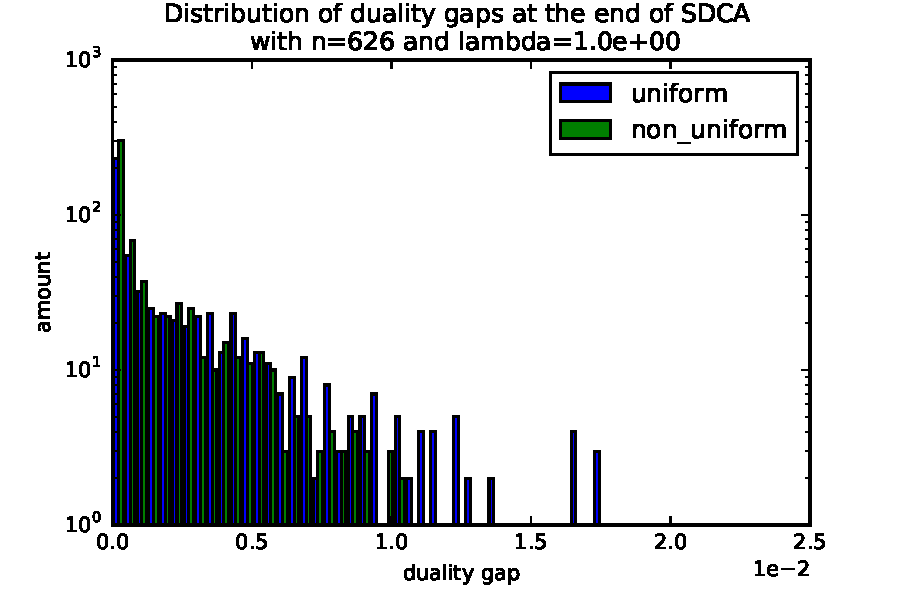
\includegraphics[width=\textwidth]{images/20170914_040308_ocr_optdualgaps.pdf}
    \end{subfigure}
    ~
    \begin{subfigure}[t]{0.3\textwidth}
        \centering
        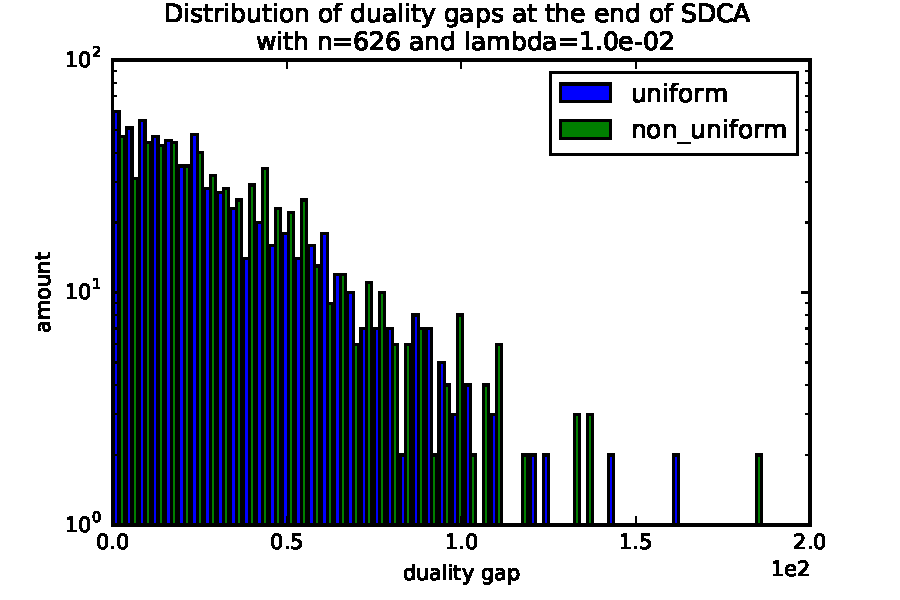
\includegraphics[width=\textwidth]{images/20170914_041703_ocr_optdualgaps.pdf}
    \end{subfigure}
    ~
    \begin{subfigure}[t]{0.3\textwidth}
        \centering
        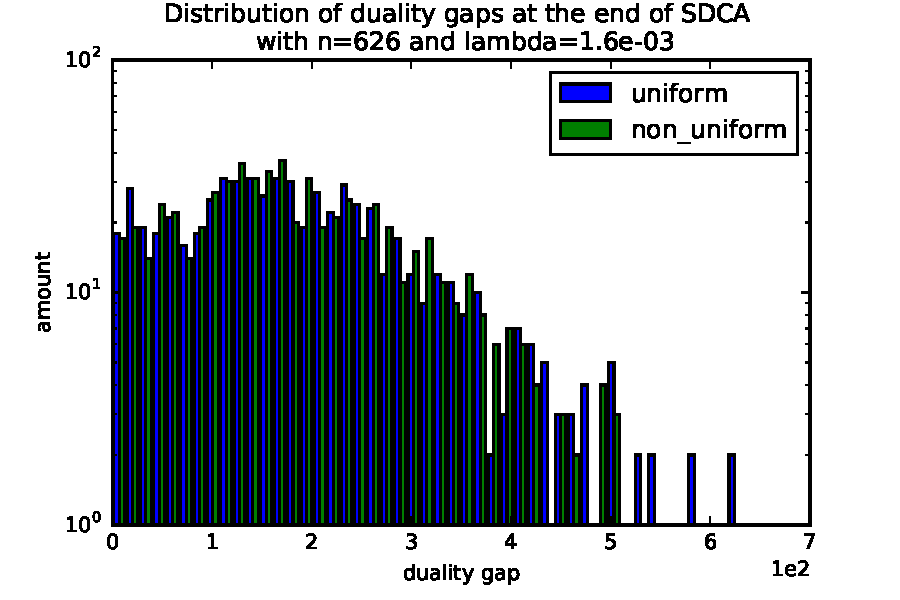
\includegraphics[width=\textwidth]{images/20170914_040725_ocr_optdualgaps.pdf}
    \end{subfigure}
    \caption{Distribution of individual duality gaps after the run of SDCA.}
	\label{ocr duality gaps}
\end{figure}
\end{frame}
%---------------------------------------------------------------------------------------
%----------------------------------------------------------------------------------------



%\begin{frame}
%\frametitle{Blocks of Highlighted Text}
%\begin{block}{Block 1}
%Lorem ipsum dolor sit amet, consectetur adipiscing elit. Integer lectus nisl, ultricies in feugiat rutrum, porttitor sit amet augue. Aliquam ut tortor mauris. Sed volutpat ante purus, quis accumsan dolor.
%\end{block}
%
%\begin{block}{Block 2}
%Pellentesque sed tellus purus. Class aptent taciti sociosqu ad litora torquent per conubia nostra, per inceptos himenaeos. Vestibulum quis magna at risus dictum tempor eu vitae velit.
%\end{block}
%
%\begin{block}{Block 3}
%Suspendisse tincidunt sagittis gravida. Curabitur condimentum, enim sed venenatis rutrum, ipsum neque consectetur orci, sed blandit justo nisi ac lacus.
%\end{block}
%\end{frame}

%------------------------------------------------

%\begin{frame}
%\frametitle{Multiple Columns}
%\begin{columns}[c] % The "c" option specifies centered vertical alignment while the "t" option is used for top vertical alignment
%
%\column{.45\textwidth} % Left column and width
%\textbf{Heading}
%\begin{enumerate}
%\item Statement
%\item Explanation
%\item Example
%\end{enumerate}
%
%\column{.5\textwidth} % Right column and width
%Lorem ipsum dolor sit amet, consectetur adipiscing elit. Integer lectus nisl, ultricies in feugiat rutrum, porttitor sit amet augue. Aliquam ut tortor mauris. Sed volutpat ante purus, quis accumsan dolor.
%
%\end{columns}
%\end{frame}
%
%%------------------------------------------------
%\section{Second Section}
%%------------------------------------------------
%
%\begin{frame}
%\frametitle{Table}
%\begin{table}
%\begin{tabular}{l l l}
%\toprule
%\textbf{Treatments} & \textbf{Response 1} & \textbf{Response 2}\\
%\midrule
%Treatment 1 & 0.0003262 & 0.562 \\
%Treatment 2 & 0.0015681 & 0.910 \\
%Treatment 3 & 0.0009271 & 0.296 \\
%\bottomrule
%\end{tabular}
%\caption{Table caption}
%\end{table}
%\end{frame}
%
%%------------------------------------------------
%
%\begin{frame}
%\frametitle{Theorem}
%\begin{theorem}[Mass--energy equivalence]
%$E = mc^2$
%\end{theorem}
%\end{frame}
%
%%------------------------------------------------
%
%\begin{frame}[fragile] % Need to use the fragile option when verbatim is used in the slide
%\frametitle{Verbatim}
%\begin{example}[Theorem Slide Code]
%\begin{verbatim}
%\begin{frame}
%\frametitle{Theorem}
%\begin{theorem}[Mass--energy equivalence]
%$E = mc^2$
%\end{theorem}
%\end{frame}\end{verbatim}
%\end{example}
%\end{frame}
%
%%------------------------------------------------
%
%\begin{frame}
%\frametitle{Figure}
%Uncomment the code on this slide to include your own image from the same directory as the template .TeX file.
%%\begin{figure}
%%\includegraphics[width=0.8\linewidth]{test}
%%\end{figure}
%\end{frame}
%
%%------------------------------------------------
%
%\begin{frame}[fragile] % Need to use the fragile option when verbatim is used in the slide
%\frametitle{Citation}
%An example of the \verb|\cite| command to cite within the presentation:\\~
%
%This statement requires citation \cite{p1}.
%\end{frame}
%
%%------------------------------------------------
%
%\begin{frame}
%\frametitle{References}
%\footnotesize{
%\begin{thebibliography}{99} % Beamer does not support BibTeX so references must be inserted manually as below
%\bibitem[Smith, 2012]{p1} John Smith (2012)
%\newblock Title of the publication
%\newblock \emph{Journal Name} 12(3), 45 -- 678.
%\end{thebibliography}
%}
%\end{frame}

%------------------------------------------------
%----------------------------------------------------------------------------------------

\end{document}